\documentclass{extarticle} % Type du document
\usepackage[french]{babel} % Langue du document
\usepackage[T1]{fontenc}
\usepackage[utf8]{inputenc}
\usepackage[left=20mm, right=20mm, top=30mm, bottom=30mm]{geometry} % Définition de la largeur des marges gauches et droites
\usepackage{a4wide} % Format de la feuille
\usepackage{amsmath} % Pour inclure des équations
\usepackage{graphicx} % Pour inclure des images / graphiques
\usepackage{float} % Pour gérer le placement des images
\usepackage{fancyhdr} % Pour les headers, paramètres ci-dessous
\usepackage{tabularx}
\usepackage{array}
\usepackage{xcolor}
\usepackage{enumitem}
\usepackage{hyperref}
\usepackage{minted}
\usepackage{url}

\definecolor{lightgray}{rgb}{0.83, 0.83, 0.83}


\pagestyle{fancy}
\lhead{Nikolaos Garanis, Nathanaël Mizutani}
\rhead{SOS - Examen Pratique}
\cfoot{\thepage}

\title{SOS - Linux\\Examen pratique}
\author{Nikolaos Garanis, Nathanaël Mizutani}
\date{18.04.2019}

\begin{document}
    \maketitle

    \bigbreak

    \tableofcontents

    \pagebreak

    \section{Résumé exécutif}
    \subsection{Mise en place de la partition chiffrée}
    Nous avons créé un espace mémoire chiffré sur l'ordinateur afin d'y sauvegarder les données du site web.
    Les données ne seront accessibles qu'au personnel autorisé à travailler sur l'ordinateur susmentionné.
    De cette façon les données seront protégées et leur accès contrôlé.

    \subsection{Restrictions}
    SELinux a été désactivé sur la machine. Ceci afin d'éviter des complications dans l'administration du système
    informatique.

    Nous avons fait en sorte que chaque utilisateur ne puisse voir que son espace de travail.
    Il ne pourra pas voir les programmes qui ne le concernent pas. Cela limite les risques en cas 
    de piratage ou face à un employé malveillant.

    De même si un utilisateur veut effectuer des actions spéciales sur l'ordinateur, il devra
    introduire son mot de passe. Ceci ajoute un niveau de protection et permet d'avoir une trace
    de qui à fait quoi.

    \subsection{Mise en place du serveur web}
    La configuration des installations pour le site web a été fait. Un système de compartimentation a été installé afin de protéger le site web.

    \subsection{Gestion des droits d'accès}
    Un système d'autorisation par défaut afin de définir qui possède le droit de faire quoi a aussi été mis en place.
    Celui-ci concerne tous les utilisateurs.

    \paragraph{Développeur web} Nous avons défini les droits pour le développeur web.
    Il est désormais autorisé à effectuer les actions nécessaires à son travail, comme mettre 
    en marche ou arrêter le site web. Par contre il ne pourra exécuter des actions qui sortent
    de son domaine de travail.


    \paragraph{Adminstrateur système} L'administrateur système possède désormais des droits privilégiés. Ce qui lui
    permettra d'effectuer toute la maintenance nécessaire sur l'ordinateur et le site web.

    \paragraph{Management} Comme demandé, le chef possède des droits nécessaires pour
     démarrer lui-même le site web. Il a accès en lecture aux données de celui-ci. 
     Il peut aussi consulter le fichier \texttt{sudoers}.

     \section{Résumé technique}

     Dans cette section nous présentons, d'une manière générale, les étapes nécessaires afin d'obtenir l'environnement demandé. Nous détaillons et expliquons aussi nos choix techniques.

     \subsection{Mise en place de la partition chiffrée}

     Les fichiers du site web sont placés dans une partition séparée de celle où est installé le système d'exploitation. 
     L'avantage est de pouvoir monter cette partition avec certaines options comme \texttt{noexec} ou \texttt{nosuid} 
     qui empêchent l'exécution des binaires présents sur la partition. En effet, il ne devrait pas y avoir de binaire
      parmi les fichiers du site web. Si un attaquant réussi à en placer un, au moins il ne pourra pas l'exécuter. La 
      partition est placée dans le deuxième disque disponible de la machine. Nous utilisons LVM (\textit{Logical Volume Manager})
       pour créer la partition.

     Nous décidons aussi de chiffrer cette partition. Cela pose une protection supplémentaire dans l'éventualité
      où un attaquant gagne un accès physique à la machine. La partition étant chiffrée elle ne peut être lue sans
       le mot de passe de déchiffrement. Pour chiffrer la partition nous utilisons la spécification LUKS 
       (\textit{Linux Unified Key Setup}) avec l'outils \texttt{cryptsetup}.

     Au démarrage de la machine, une fois le mot de passe de déchiffrement entré, 
     la partition est déchiffrée puis montée automatiquement dans le répertoire \texttt{/var/www/html}.
      Ce répertoire est celui par défaut qu'Apache va utiliser pour servir les fichiers du site web.

     \subsection{Restrictions}

     L'utilisation de SELinux, activé par défaut sur CentOS 7, requiert des compétences supplémentaires qui
      ne sont pas demandées dans le cadre de la mise en place de notre environnement. Pour cette raison, nous
       désactivons SELinux afin de ne pas avoir de problèmes dû à des éléments que nous ne maîtrisons pas.

     Nous restreignons aussi la visibilité des processus s'exécutant sur la machine. Par défaut, seul 
     l'utilisateur root pourra visualiser ces processus. Il n'est en fait pas nécessaire que certains
      utilisateurs, par exemple le développeur web, puisse voir quels processus tournent sur la machine.
       Ainsi, si cet utilisateur est compromis, l'attaquant n'aura pas accès à ces informations.

     Nous voulons aussi qu'à chaque fois qu'un utilisateur veuille lister ses droits sudo, il devra 
     entrer son mot de passe. Dans le cas ou un attaquant accède à un compte utilisateur sans pour 
     autant en connaître le mot de passe, il ne pourra pas voir les droits sudo qu'il possède. C'est 
     une protection supplémentaire contre la recherche de vulnérabilités dans les droits sudo.

     \subsection{Mise en place du serveur web}

     Le site web sera servi par un serveur Apache, lequel tournera dans un conteneur Docker. Pour que 
     les pages dynamiques en PHP soient supportées, nous utilisons l’image Docker \texttt{php:apache} 
     fournie par PHP. Le choix de cette image nous évite toute configuration relative à PHP et Apache. 
     L'utilisation d'un conteneur Docker permet de rajouter une barrière de protection supplémentaire 
     dans l'éventualité d'une compromission du serveur web.

     Afin que le conteneur soit lancé au démarrage de la machine, nous créons un service systemd. 
     Celui-ci lancera le conteneur avec les options nécessaires pour mapper le port 80 du conteneur 
     au port 8080 de la machine et pour monter \texttt{/var/www/html} à l'intérieur du container. 
     Le répertoire est monté en lecture seule, ce qui empêche toutes modifications des fichiers 
     du site web depuis le conteneur. Les options spécifient aussi le nom et \textit{hostname} 
     qu'aura le conteneur une fois démarré, ainsi que sa suppression automatique une fois arrêté.

     Afin de tester l'installation, une page PHP de test est créée à la racine du site web (sur 
     la machine hôte). Cette page affiche simplement le \textit{hostname} du conteneur.

     Nous voulons que les requêtes HTTP, donc arrivant sur le port 80 de la machine, soient 
     redirigées vers son port 8080. Celui-ci étant associé au port 80 du conteneur, les 
     requêtes seront délivrées jusqu'au serveur Apache tournant dans le conteneur. Pour 
     ce faire, deux règles iptables sont nécessaires, une pour rediriger vers le port 8080 
     le trafic à destination du port 80, et la deuxième pour accepter le trafic à destination 
     du port 8080. Ces deux règles doivent bien entendu être persistantes et donc être chargées 
     au démarrage de la machine.

     \subsection{Gestion des droits d'accès}

     Ont accès à la machine trois utilisateurs (qui doivent être créés), chacun avec des 
     droits distincts, adaptés à leur fonction. L'utilisateur devuser, s'occupant du 
     développement web, a la possibilité de faire un \texttt{pull} de l'image Docker 
     mentionnée plus haut. Il doit aussi pouvoir (re)démarrer, arrêter et activer le service 
     systemd créé. Ces droits sont spécifiés dans un nouveau fichier sudoers, réservé à cet 
     utilisateur. Nous utilisons aussi les ACL afin de donner les droits de lecture et d'écriture  
     pour le fichier \texttt{/etc/hosts} ainsi que tous les fichiers dans \texttt{/var/www/html}.

     L'utilisateur sysuser gère l'administration de la machine, il possède des privilèges plus élevés. 
     Tout d'abord, il doit appartenir aux groupes wheel et docker. Ensuite, tout comme devuser, il 
     peut lire et modifier tous les fichiers du site web. En plus de cela, l'utilisateur doit pouvoir 
     exécuter n'importe quelle commande en tant que root. Ceci demande la création d'un nouveau fichier 
     sudoers contenant les droits appropriés. Nous voulons aussi que l'utilisateur puisse voir tous les 
     processus tournant sur la machine. Il nous faut pour cela utiliser l'option \texttt{gid}, qui permet 
     de faire une exception à l'option \texttt{hidepid} que nous avons utiliser précédemment pour le 
     montage de la partition du système de fichier \texttt{/proc}.

     Quant à l'utilisateur bossuser, il possède des droits restreints. Il ne peut que lire les fichiers 
     du site web et non pas les modifier. Comme pour les autres utilisateurs, nous gérons ces droits en 
     utilisant les ACL. Les commandes que peut effectuer l'utilisateur sont aussi restreintes, il ne peut 
     que démarrer et arrêter le service du conteneur. Un nouveau fichier sudoers est créé pour cela. 
     Additionnellement, nous voulons que l'utilisateur puisse lire le fichier \texttt{/etc/sudoers}. Les 
     ACL sont utilisées pour ce faire.

    \section{Détail des manipulations}

    Nous présentons dans cette section les commandes effectuées ainsi que les fichiers de configuration nécessaires à la mise en place du site web.
     Nous prenons comme base la machine virtuelle fournie lors du cours de \textit{Sécurité des Systèmes d'Exploitation} (SOS). Notre environnement
      possède alors les caractéristiques suivantes :

    \begin{enumerate}[label=$\bullet$]
      \item système d'exploitation CentOS 7,
      \item utilisateur possédant les droits administrateurs,
      \item disque libre sur lequel seront mis les fichiers du site web,
      \item Docker installé.
    \end{enumerate}

    \subsection{Mise en place de la partition chiffrée}

    \subsubsection{Création, chiffrement et formatage}

    Afin d'initialiser la partition nous utilisons LVM (\textit{Logical Volume Manager}). Nous commençons par créer un \textit{volume physique}
    sur le deuxième disque de la machine (\texttt{/dev/sdb} dans notre cas).

    \begin{minted}[style=friendly, bgcolor=lightgray]{bash}
    $ sudo pvcreate /dev/sdb
    \end{minted}

    Puis, il est nécessaire de créer un \textit{groupe virtuel} dans le volume initialisé ci-dessus. Nous le nommons \texttt{vg-site}.

    \begin{minted}[style=friendly, bgcolor=lightgray]{bash}
    $ sudo vgcreate vg-site /dev/sdb
    \end{minted}

    Nous créons maintenant un \textit{volume logique} à l'intérieur du groupe \texttt{vg-site} occupant 100\% de l'espace disponible. Nous le nommons \texttt{lv-site}.

    \begin{minted}[style=friendly, bgcolor=lightgray]{bash}
    $ sudo lvcreate -l100%FREE vg-site -n lv-site
    \end{minted}

    Nous utilisons ensuite LUKS (\textit{Linux Unified Key Setup}) pour chiffrer la partition, étape à laquelle il nous est
    demandé d'entrer le mot de passe pour chiffrer la partition, nous utilisons \texttt{vg-site123;}.

    \begin{minted}[style=friendly, bgcolor=lightgray]{bash}
    $ sudo cryptsetup luksFormat /dev/vg-site/lv-site
    \end{minted}

    Il faut maintenant déchiffrer la partition afin de la formatter en \texttt{ext4}.

    \begin{minted}[style=friendly, bgcolor=lightgray]{bash}
    $ sudo cryptsetup open --type luks /dev/vg-site/lv-site site-crypt
    $ sudo mkfs.ext4 /dev/mapper/site-crypt
    \end{minted}

    \subsubsection{Déchiffrement et montage au démarrage de la machine}

    Afin que la partition soit déchiffrée au démarrage de la machine, une entrée doit être ajoutée dans le fichier \texttt{/etc/crypttab}.

    \begin{minted}[style=friendly, bgcolor=lightgray]{bash}
    $ echo "site-crypt /dev/vg-site/lv-site none" | sudo tee -a /etc/crypttab
    \end{minted}

    \begin{figure}[H]
      \centering
      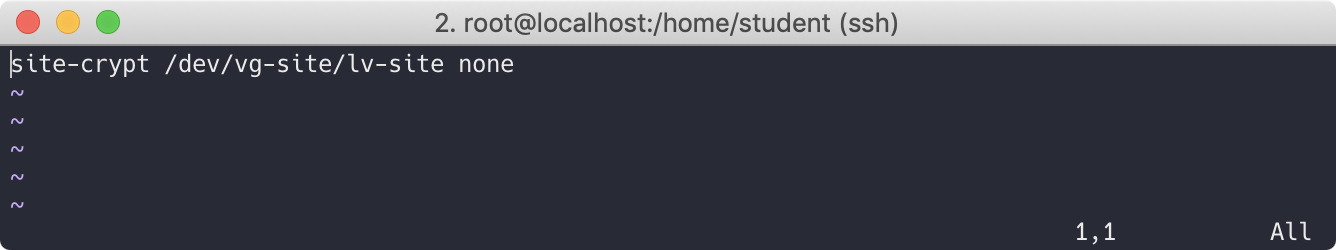
\includegraphics[scale=0.6]{img/crypttab.png}
      \caption{Contenu du fichier \texttt{crypttab}}
    \end{figure}

    Une entrée doit aussi être ajoutée au fichier \texttt{/etc/fstab} pour que la partition déchiffrée soit montée
     automatiquement dans \texttt{/var/www/html} avec les options \texttt{nosuid} et \texttt{noexec}.

    \begin{minted}[style=friendly, bgcolor=lightgray]{bash}
    $ echo "/dev/mapper/site-crypt /var/www/html ext4 defaults,noexec,nosuid 0 0" \
      | sudo tee -a /etc/fstab
    \end{minted}

    \begin{figure}[H]
      \centering
      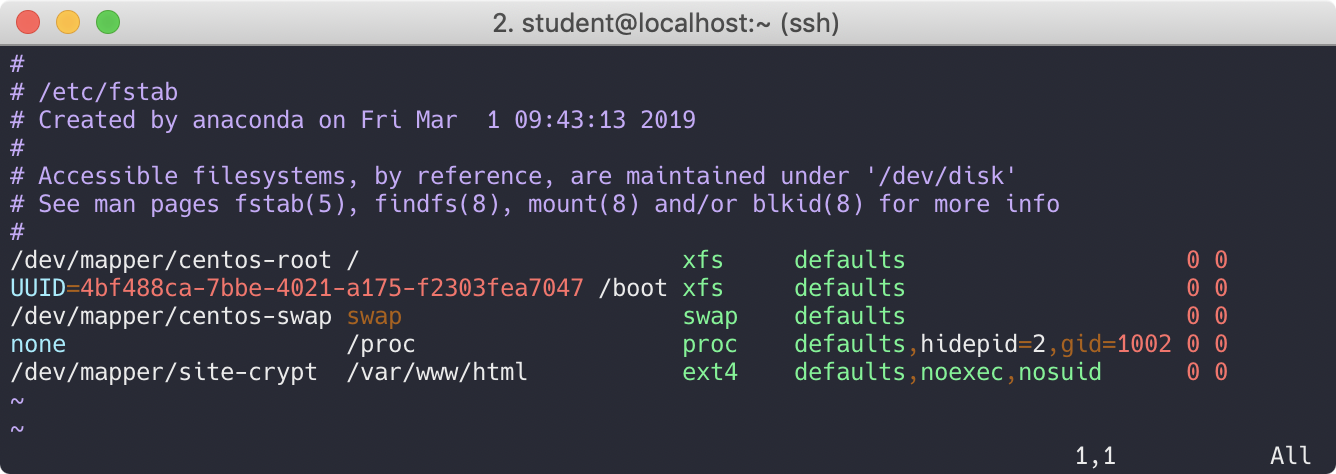
\includegraphics[scale=0.6]{img/fstab.png}
      \caption{Contenu du ficher \texttt{fstab}}
    \end{figure}

    \subsection{Restrictions}
    \subsubsection{Désactivation de SELinux}

    Pour désactiver SELinux il faut éditer le fichier \texttt{/etc/sysconfig/selinux} et y changer la valeur
     de la variable \texttt{SELINUX} à \texttt{disabled}. Afin que le changement soit pris en compte la machine doit être redémarrée.

    \begin{minted}[style=friendly, bgcolor=lightgray]{bash}
    $ sudo sed -i -E 's/^(SELINUX=).*$/\1disabled/' /etc/sysconfig/selinux
    $ reboot
    $ sestatus
    SELinux status:                 disabled
    \end{minted}

    \subsubsection{Masquage des processus}

    Pour empêcher les utilisateurs de voir les processus qui tournent sur le système il nous faut modifier
    le fichier \texttt{/etc/fstab} afin d'y ajouter une entrée pour le système de fichier \texttt{/proc},
    celui-ci doit être monté avec l'option \texttt{hidepid}. Pour que la modification prenne effet, il faut le remonter.

    \pagebreak
    \begin{minted}[style=friendly, bgcolor=lightgray]{bash}
    $ echo -e "none /proc proc defaults,hidepid=2 0 0" | sudo tee -a /etc/fstab
    $ sudo mount -o remount /proc

    # vérification
    $ mount | grep hidepid=2
    proc on /proc type proc (rw,nosuid,nodev,noexec,relatime,hidepid=2)
    \end{minted}

    \subsubsection{Demande du mot de passe pour \texttt{sudo -l}}

    Afin que le mot de passe d'un utilisateur exécutant la commande \texttt{sudo -l} lui soit toujours demandé, nous créons le fichier \texttt{/etc/sudoers.d/general}.

    \begin{minted}[style=friendly, bgcolor=lightgray]{bash}
    $ echo Defaults listpw=always | sudo tee /etc/sudoers.d/general
    \end{minted}

    \subsubsection{Droits d'accès pour \texttt{/etc/sudoers*}}

    Les droits en lecture du fichier \texttt{/etc/sudoers} ne doivent être attribués qu'à l'utilisateur root.

    \begin{minted}[style=friendly, bgcolor=lightgray]{bash}
    $ sudo chmod 400 /etc/sudoers
    \end{minted}

    Afin de faire de même avec tous les fichiers qui seront créés dans le répertoire \texttt{/etc/sudoers.d}, nous lui attribuons des ACL par défaut.

    \begin{minted}[style=friendly, bgcolor=lightgray]{bash}
    $ sudo setfacl -d -m u::r,g::-,o::- /etc/sudoers.d
    \end{minted}

    \subsection{Mise en place du serveur web}
    \subsubsection{Création d'un service systemd}

    Nous définissons un service systemd qui s'occupe de lancer et d'arrêter le conteneur Docker dans lequel
    tourne le serveur Apache. Pour cela, nous créons le fichier \texttt{/etc/systemd/system/httpd-php-container.service} avec le contenu suivant :

    \begin{minted}[style=friendly, bgcolor=lightgray]{bash}
    [Unit]
    Description=httpd-php-container

    [Service]
    Restart=always
    ExecStart=/usr/bin/docker run --rm --name httpd-php-container --hostname \
    httpd-php-container -p 8080:80 -v /var/www/html:/var/www/html:ro php:apache
    ExecStop=/usr/bin/docker container kill httpd-php-container

    [Install]
    WantedBy=multi-user.target
    \end{minted}

    \begin{figure}[H]
      \centering
      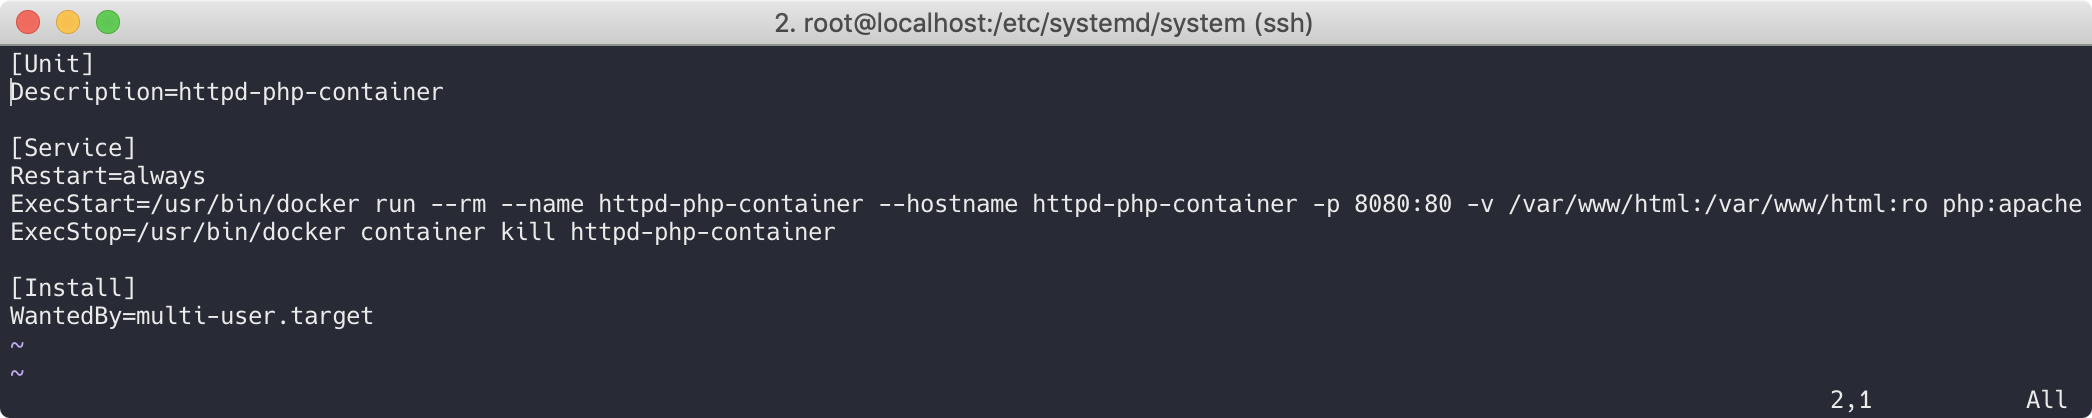
\includegraphics[scale=0.45]{img/systemd.png}
      \caption{Contenu du fichier \texttt{httpd-php-container.service}}
    \end{figure}

    Il nous faut maintenant activer le service afin que celui-ci se lance au démarrage 
    de la machine (l'option \texttt{--now} permet en plus de le lancer immédiatement) :

    \begin{minted}[style=friendly, bgcolor=lightgray]{bash}
    $ sudo systemctl enable --now httpd-php-container
    \end{minted}

    \subsubsection{Création d'une page web PHP}

    Dans le répertoire \texttt{/var/www/html} de la machine, nous créons une page test en PHP affichant 
    le hostname du conteneur.

    \begin{minted}[style=friendly, bgcolor=lightgray]{bash}
    $ echo "<?php echo 'Hello from: '. gethostname() .\"\n\"; ?>" \
      | sudo tee /var/www/html/index.php
    \end{minted}

    \subsubsection{Gestion des règles iptables}

    Afin de rediriger le trafic entrant sur le port 80 de la machine vers le
    port 8080 de celle-ci, nous ajoutons une règle iptables dans la chaîne \texttt{PREROUTING} de la table \texttt{nat}.

    \begin{minted}[style=friendly, bgcolor=lightgray]{bash}
    $ sudo iptables -t nat -A PREROUTING -p tcp --dport 80 -j REDIRECT --to-port 8080
    \end{minted}

    Nous devons aussi accepter le trafic entrant sur le port 8080 de la machine.

    \begin{minted}[style=friendly, bgcolor=lightgray]{bash}
    $ sudo iptables -I INPUT -p tcp --dport 8080 -j ACCEPT
    \end{minted}

    Afin de rendre ces règles persistantes, nous les sauvegardons dans le fichier \texttt{/etc/sysconfig/iptables}.

    \begin{minted}[style=friendly, bgcolor=lightgray]{bash}
    $ sudo iptables-save | sudo tee /etc/sysconfig/iptables
    \end{minted}

    Puis, il nous faut créer le script \texttt{/sbin/ifup-local} qui sera exécuté à chaque fois qu'une
     interface réseau sera activée. Le fichier doit être exécutable et son contenu est le suivant :

    \begin{minted}[style=friendly, bgcolor=lightgray]{bash}
    $ sudo chmod +x /sbin/ifup-local
    $ cat /sbin/ifup-local
    #!/usr/bin/env sh
    iptables-restore < /etc/sysconfig/iptables
    \end{minted}

    \pagebreak
    \subsection{Gestion des droits d'accès}
    \subsubsection{Utilisateur devuser}

    \paragraph{Création} Nous commençons par créer l'utilisateur devuser :

    \begin{minted}[style=friendly, bgcolor=lightgray]{bash}
    $ sudo useradd -m -s /bin/bash devuser
    \end{minted}

    \paragraph{Droits sudo} Afin que l'utilisateur puisse télécharger l'image Docker \texttt{php:apache}
     ainsi que (re)démarrer, arrêter et activer le service \texttt{httpd-php-container}, nous lui autorisons
     ces actions dans le fichier \texttt{/etc/sudoers.d/devuser} que nous créons avec le contenu suivant :

    \begin{minted}[style=friendly, bgcolor=lightgray]{bash}
    devuser ALL = /usr/bin/docker pull php:apache,                \
                  /usr/bin/systemctl start httpd-php-container,   \
                  /usr/bin/systemctl stop httpd-php-container,    \
                  /usr/bin/systemctl restart httpd-php-container, \
                  /usr/bin/systemctl enable httpd-php-container
    \end{minted}

    \begin{figure}[H]
      \centering
      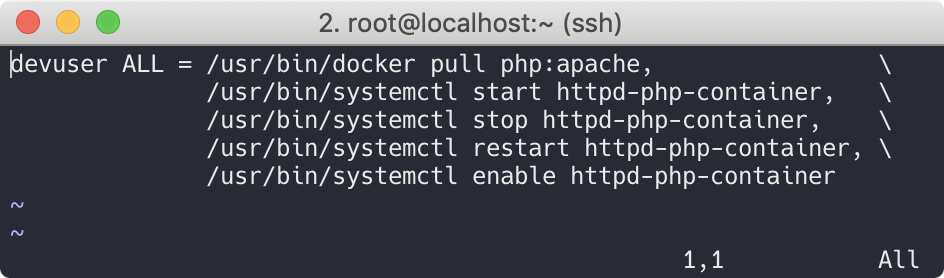
\includegraphics[scale=0.7]{img/devuser.png}
      \caption{Contenu du fichier \texttt{devuser}}
    \end{figure}

    \paragraph{ACL} L'utilisateur doit aussi pouvoir lire et écrire tous les fichiers présents et futurs dans
     \texttt{/var/www/html}. Pour les fichiers déjà présents, ou pour ceux qui seront déplacés dans ce répertoire,
      nous appliquons les ACL de manière récursive.

    \begin{minted}[style=friendly, bgcolor=lightgray]{bash}
    $ sudo setfacl -R -m u:devuser:rw- /var/www/html
    \end{minted}

    Pour les fichiers qui seront créés dans le répertoire, nous lui attribuons des ACL par défaut.

    \begin{minted}[style=friendly, bgcolor=lightgray]{bash}
    $ sudo setfacl -d -m u:devuser:rw- /var/www/html
    \end{minted}

    Afin que l’utilisateur puisse modifier le fichier \texttt{/etc/hosts}, nous appliquons les ACL suivantes :

    \begin{minted}[style=friendly, bgcolor=lightgray]{bash}
    $ sudo setfacl -m u:devuser:rw- /etc/hosts
    \end{minted}


    \subsubsection{Utilisateur sysuser}

    \paragraph{Création} Nous créons l'utilisateur sysuser et nous l'ajoutons directement dans les groupes wheel et docker :

    \begin{minted}[style=friendly, bgcolor=lightgray]{bash}
    $ sudo useradd -m -s /bin/bash -G wheel,docker sysuser
    \end{minted}

    \paragraph{Droits sudo} Pour autoriser à l'utilisateur tous les droits sudo sans aucune restriction, nous créons le fichier \texttt{/etc/sudoers.d/sysuser}.

    \begin{minted}[style=friendly, bgcolor=lightgray]{bash}
    $ echo sysuser ALL = (ALL) ALL | sudo tee /etc/sudoers.d/sysuser
    \end{minted}


    \paragraph{ACL} Afin qu'il puisse modifier les fichiers du site web nous appliquons les mêmes ACL que pour l'utilisateur devuser :

    \begin{minted}[style=friendly, bgcolor=lightgray]{bash}
    $ sudo setfacl -R -m u:sysuser:rw- /var/www/html
    $ sudo setfacl -d -m u:sysuser:rw- /var/www/html
    \end{minted}

    \paragraph{Exception \texttt{hidepid}} Nous avons précédement ajouter l'option de montage \texttt{hidepid}
    au système de fichiers \texttt{/proc}. Afin que cette option ne s'applique pas à l'utilisateur, nous devons
     rajouter l'option \texttt{gid} à l'entrée \texttt{/etc/fstab} de \texttt{/proc}. La valeur à utiliser est
      l'id du groupe principal auquel appartient sysuser.

    \begin{minted}[style=friendly, bgcolor=lightgray]{bash}
    $ id -g sysuser
    1002 # par exemple

    # contenu de l'entrée après modification
    $ cat /etc/fstab | grep /proc
    none /proc proc defaults,hidepid=2,gid=1002 0 0

    # appliquer le changement
    $ sudo mount -o remount /proc
    \end{minted}

    \begin{figure}[H]
      \centering
      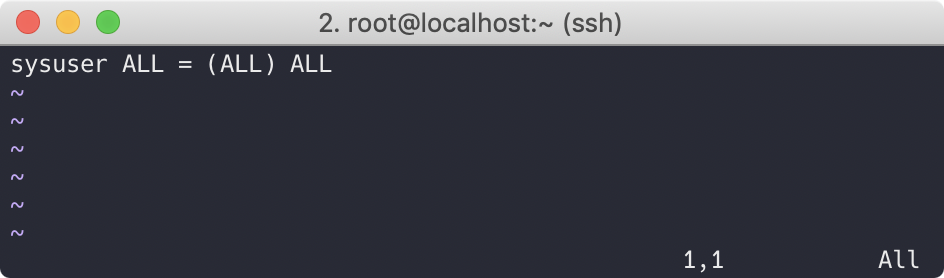
\includegraphics[scale=0.7]{img/sysuser.png}
      \caption{Contenu du fichier \texttt{sysuser}}
    \end{figure}

    \subsubsection{Utilisateur bossuser}

    \paragraph{Création} Nous commençons par créer l'utilisateur bossuser :

    \begin{minted}[style=friendly, bgcolor=lightgray]{bash}
    $ sudo useradd -m -s /bin/bash bossuser
    \end{minted}

    \paragraph{Droits sudo} L’utilisateur doit pouvoir arrêter et démarrer le service systemd créé précédement,
    pour cela nous créons le fichier \texttt{/etc/sudoers.d/bossuser} avec le contenu suivant :

    \begin{minted}[style=friendly, bgcolor=lightgray]{bash}
    bossuser ALL = /usr/bin/systemctl start httpd-php-container, \
                   /usr/bin/systemctl stop httpd-php-container
    \end{minted}

    \begin{figure}[H]
      \centering
      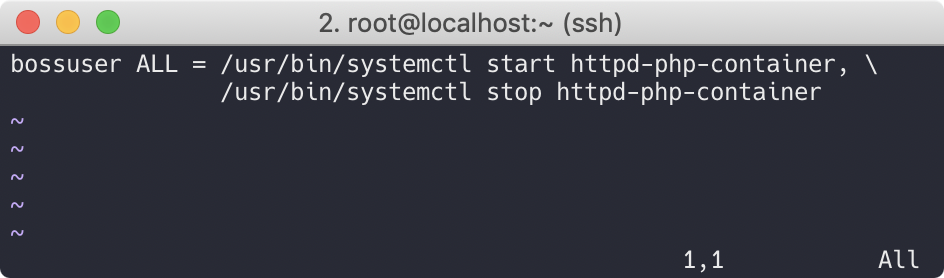
\includegraphics[scale=0.7]{img/bossuser.png}
      \caption{Contenu du fichier \texttt{bossuser}}
    \end{figure}

    \paragraph{ACL} Pour que l’utilisateur puisse seulement lire les fichiers du site web, nous utilisons les
    ACL par défaut sur le répertoire. Nous appliquons aussi les ACL de manière récursive pour les fichiers déjà présents.

    \begin{minted}[style=friendly, bgcolor=lightgray]{bash}
    $ sudo setfacl -R -m u:bossuser:r-- /var/www/html
    $ sudo setfacl -d -m u:bossuser:r-- /var/www/html
    \end{minted}

    L’utilisateur doit aussi pouvoir lire le fichier \texttt{/etc/sudoers}, nous utilisons encore une fois les ACL :

    \begin{minted}[style=friendly, bgcolor=lightgray]{bash}
    $ sudo setfacl -m u:bossuser:r-- /etc/sudoers
    \end{minted}

    \section{Sources}

    \begin{enumerate}[label=>]
      \item \url{https://www.vmotionhost.com/client-area/knowledgebase.php?action=displayarticle&id=163}
      \item \url{https://www.tecmint.com/disable-selinux-temporarily-permanently-in-centos-rhel-fedora/}
      \item \url{https://linux-audit.com/linux-system-hardening-adding-hidepid-to-proc/}
      \item \url{https://www.sudo.ws/man/1.8.27/sudoers.man.html}
      \item \url{https://hub.docker.com/_/httpd}
      \item \url{https://hub.docker.com/_/php/}
    \end{enumerate}

\end{document}
